\documentclass[12pt]{article}

\usepackage{sbc-template}
\usepackage{graphicx,url}
\usepackage[utf8]{inputenc}
\usepackage[brazil]{babel}
     
\sloppy

\title{EASYCODE: UM AMBIENTE DE TECNOLOGIAS DE APOIO PARA O ENSINO DE LÓGICA DE PROGRAMAÇÃO}

\author{Daniela F. Feitosa \inst{1}, Eduardo N. B. Neves \inst{2}, Jucimar B. Souza \inst{1}, Emmerson S. R. Silva \inst{3} }

\address{Instituto Federal de Educação, Ciência e Tecnologia do Amazonas \\ Campus Manaus Centro (IFAM-CMC)
  \email{\{danielaferreira1133, eddunic, jucibs, emmsr2004\}@gmail.com}
}

\begin{document} 

\maketitle

\begin{abstract}
\end{abstract}
     
\begin{resumo}
Este plano de pesquisa apresenta a contribuição científica objetivada para o software EasyCode, desenvolvido por alunos do IFAM-CMC em 2017, visando adequá-lo aos estudantes que têm dificuldade em aplicar a lógica de programação do paradigma imperativo na resolução de problemas computacionais. Consistirá na aplicação do domínio cognitivo da Taxonomia de Bloom Revisada (ANDERSON et al., 2001) em conjunto com representações gráficas (fluxogramas e simuladores de aspectos da vertente educacional em estudo), gamificação baseada nas categorias do referido domínio da taxonomia, e da robótica educacional a fim de proporcionar a compreensão de problemas computacionais de acordo com os tipos de aprendizagem. Objetiva-se incentivo ao aprendizado de linguagens da programação imperativa. A aplicação deste conjunto de métodos no processo de ensino-aprendizagem permitirá que conceitos da programação sejam compreendidos de maneira lúdica.
\end{resumo}

\section{Introdução}
As dificuldades apresentadas no ensino de programação variam desde a abordagem utilizada para o ensino, à possíveis barreiras para a acessibilidade ou aspectos psicológicos. Dentre o conjunto de fatores que inviabilizam a compreensão da programação apontados por Gomes \textit{et al}. (2008), destacam-se a falta de motivação e a complexidade das linguagens de programação utilizadas em conjunto com o 	desenvolvimento da lógica.

\section{Metodologia}

\section{Resultados e Discussão}
	\begin{figure}[h]
		\centering
		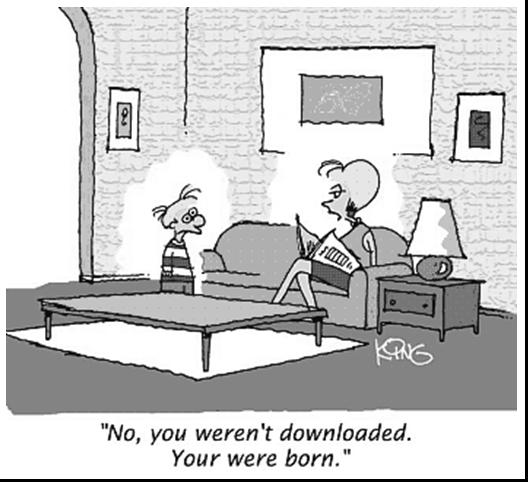
\includegraphics[scale=0.2]{fig1.jpg}
		\caption{Uma típica figura.}
		\label{fig1}
	\end{figure}

\section{Considerações Finais}

\cite{SILVA:2017}

\bibliographystyle{sbc}
\bibliography{ArtigoEC}

\end{document}